\chapter{External Validity}

Chapters 4--6 use synthetic graphs and a synthetic error knob. Is the
picture real? We stress it three ways, each replacing one synthetic
ingredient with its real counterpart: §7.1 replaces the synthetic error
with genuine temporal drift from a real request trace, §7.2 replaces the
synthetic graphs with six real ones, and §7.3 replaces the hand-made
predictor with a learned one.

\section{A real, cheap predictor}

We replace the synthetic knob with the cheapest realistic predictor:
last-window historical statistics. Real Wikipedia daily pageviews give a
live day (the truth) and earlier days (a 1-, 7-, or 30-day-stale
forecast), so the error is genuine temporal drift; we map the trace onto
a fixed serving topology and consume the forecast through the degree
route (MPD) (\textbf{Figure 7.1}). Throughout this chapter we measure
how much of the available benefit a predictor realizes by its
\textbf{gap-capture},
\((\rho_{\mathrm{ALG}}-\rho_{\mathrm{base}})/(\rho_{\mathrm{oracle}}-\rho_{\mathrm{base}})\)
, the fraction of the baseline-to-oracle gap it closes. Three facts
emerge.

First, \textbf{the predictor is cheap}. The with-predictions literature
usually pictures an expensive learned model; here it is a linear-time
count, about \(0.11\) ms per instance against \(4.4\) ms to compute
\(\mathrm{OPT}\) once, a few percent. These are the only wall-clock
numbers in the thesis and are therefore machine-dependent; everything
else is a ratio.

Second, \textbf{the benefit is real, partial, and never harmful}: a
stale forecast reaches \(27\%\)--\(68\%\) gap-capture (falling with
staleness) and always stays above the baseline (\(0.938\)--\(0.957\) vs
\(0.923\)--\(0.925\), even at 30 days).

Third, and this is why: \textbf{topology aggregation makes the cheap
predictor order-faithful}. The induced degree predictor's order error is
only Kendall-\(\tau\approx0.19\)--\(0.32\), roughly half the raw
histogram's (\(0.38\)--\(0.49\)), and since MPD depends only on order
(Chapter 5), the aggregated route survives real drift. Consuming the
\emph{same} forecast through the raw histogram is catastrophic: blind
FollowPrediction collapses to \(0.68\to0.36\), far below the
\(\approx0.92\) baseline: exactly what the robust algorithms of Chapters
4 and 6 are for.

\begin{figure}
\centering
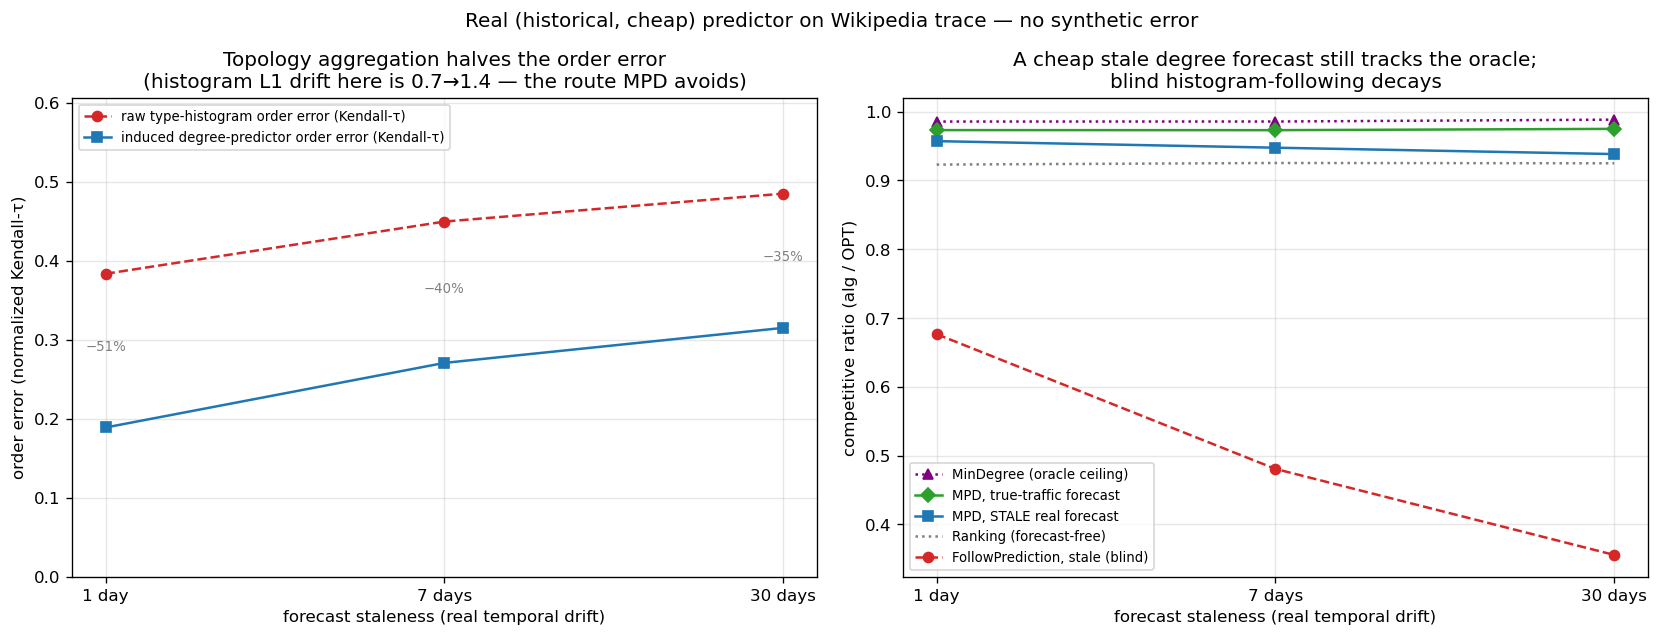
\includegraphics[width=0.8\linewidth,height=\textheight,keepaspectratio,alt={The figure to remember from this chapter: a real, cheap predictor (Wikipedia trace). The aggregated degree route survives staleness (b) because aggregation halves the order error (a); blind histogram-following decays.}]{../../results/real_predictor.png}
\caption{The figure to remember from this chapter: a real, cheap
predictor (Wikipedia trace). The aggregated degree route survives
staleness (b) because aggregation halves the order error (a); blind
histogram-following decays.}
\end{figure}

\section{Six real-world graphs}

We re-run the degree-prediction roster of Chapter 4 on the six
Network-Repository graphs (two Facebook social, two C. elegans
biological, two economic input-output), across the same quality columns,
with 95\% CIs (\textbf{Figure 7.2}). The two load-bearing findings are
universal. \textbf{F1 holds on all six}: naive MPD fed an adversarial
predictor falls below the Ranking floor everywhere, by \(0.06\) (Reed98)
to \(0.10\) (CE-PG). \textbf{F3 holds on all six, and confirms its own
logic}: the consistency upside is small everywhere (mean \(+0.049\);
range \(+0.022\)--\(+0.077\)) and smallest exactly where the baseline is
strongest: the two dense economic graphs, with Ranking already
\(0.965\)/\(0.977\), give the tiniest upsides.

The structural-robustness finding \textbf{F2 holds qualitatively on all
six} (the augmentations' spread across quality columns is smaller than
naive MPD's on every graph) and \emph{strictly}, by the stronger
criterion that the spread is at most half of MPD's, on the four
social/bio graphs (spread \(0.22\)--\(0.29\times\) MPD's); on the two
dense economic graphs the protection is only \emph{partial}: the
augmentation cushions the adversarial drop (\(0.939\) vs naive MPD's
\(0.893\)) but cannot clear the unusually high \(0.965\) floor, dipping
\(\approx0.03\) below it. Those two graphs are so dense that matching is
nearly trivial (Ranking \(\approx0.97\), MinDegree \(=1.00\)), so there
is neither upside to capture (F3) nor much downside to protect: the
boundary is F3's own mechanism at work, not an exception to it. Finally,
F4 is dramatic: the worst-case-designed Feldman/Jaillet--Lu are the
weakest advice-free entries on the econ graphs (\(0.73\)--\(0.77\)) and
the augmentation lifts them to \(0.99\), a \(+0.26\) rescue.

\begin{figure}
\centering
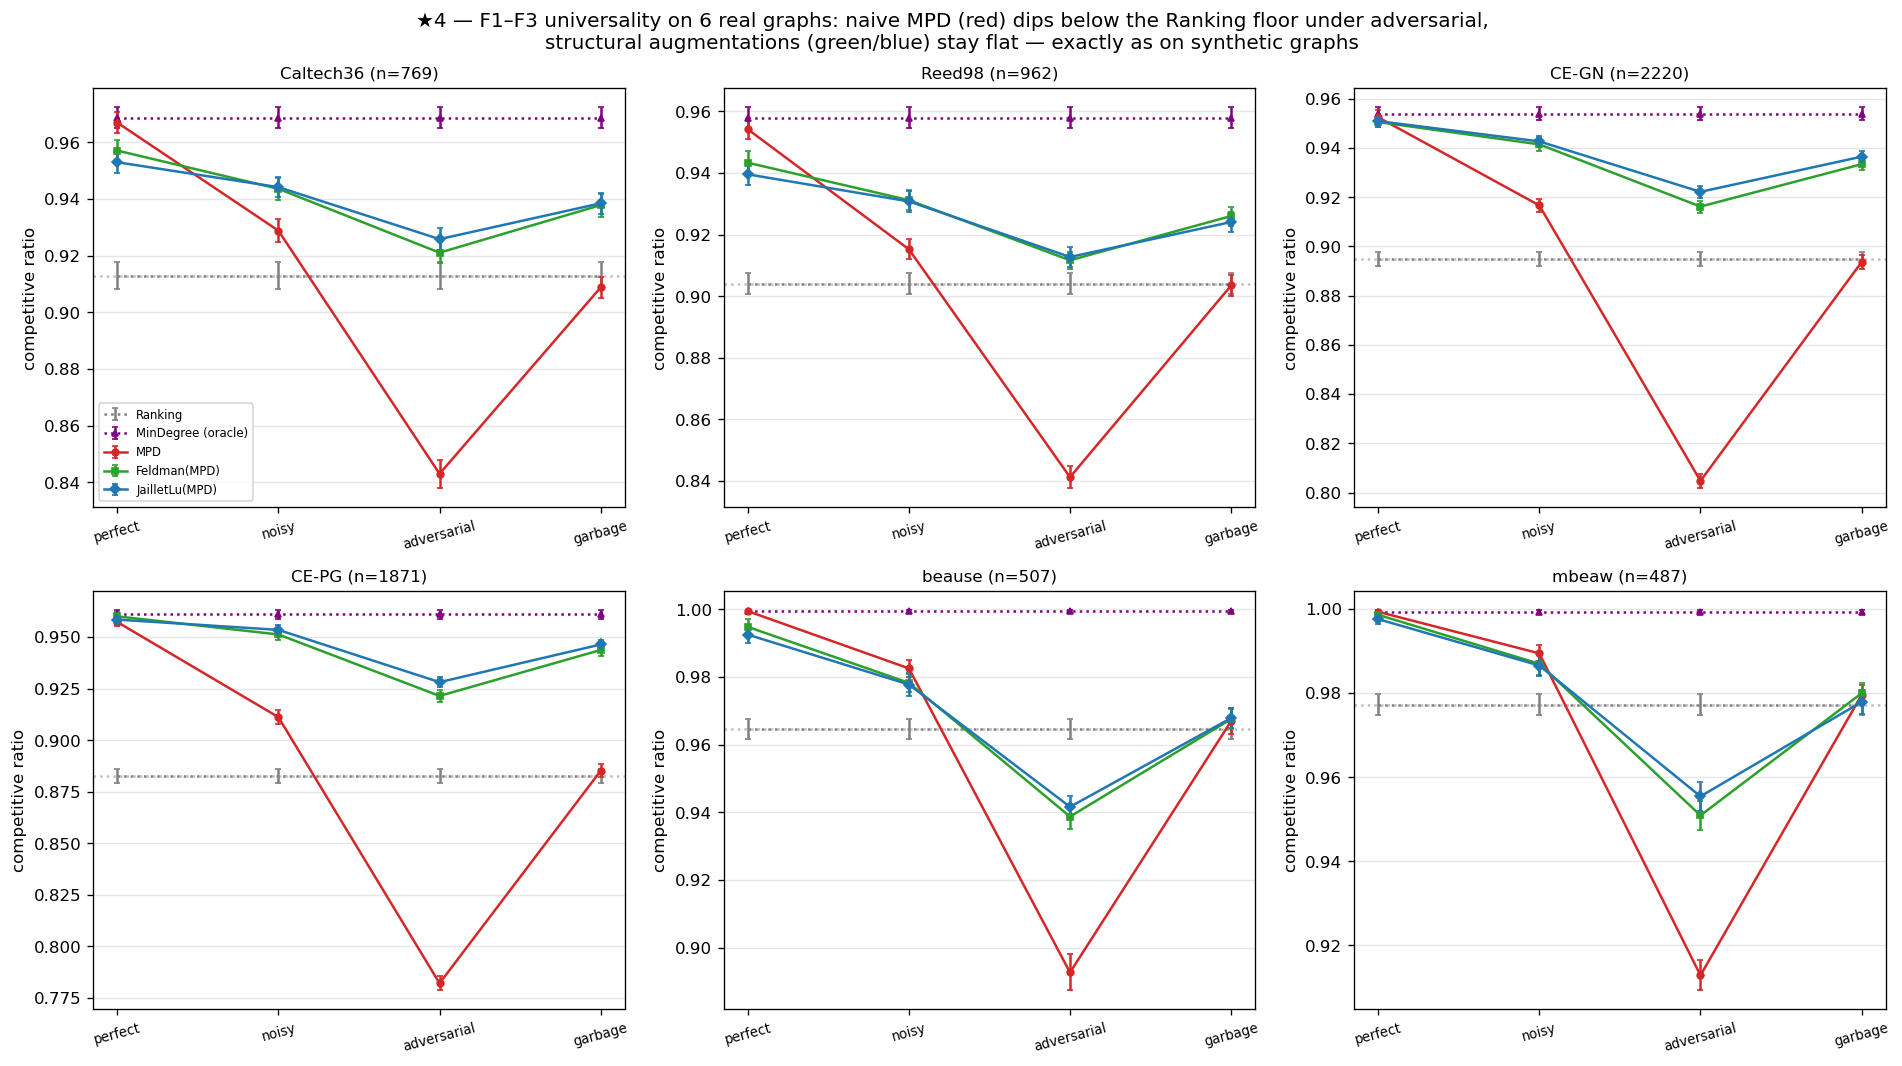
\includegraphics[width=1\linewidth,height=\textheight,keepaspectratio,alt={F1--F3 on six real graphs, one panel per graph (axis ranges differ between panels, as the graphs' floors do too, so read each panel against its own dashed floor rather than across panels). Naive MPD (red) dips below the Ranking floor everywhere; the structural augmentations (green/blue) stay flat.}]{../../results/realworld_robustness.png}
\caption{F1--F3 on six real graphs, one panel per graph (axis ranges
differ between panels, as the graphs' floors do too, so read each panel
against its own dashed floor rather than across panels). Naive MPD (red)
dips below the Ranking floor everywhere; the structural augmentations
(green/blue) stay flat.}
\end{figure}

\section{Does learning the predictor
help?}

Because MPD consumes the predictor only through order (Chapter 5), one
might train it with a rank loss rather than regression. We tested this
and report an honest negative: the advantage is real on deliberately
engineered features but disappears on real temporal ones, where rank-
and regression-trained predictors induce the same order and reach the
same ratio. The experiments, their numbers and the three-step argument
behind them are in §8.1; what matters for external validity is only the
consequence. Once a predictor is order-faithful, which a cheap
historical count already is (§7.1), neither a better algorithm nor a
better-trained predictor buys much on average-case matching.

\section{Chapter summary}

On real predictors, real graphs, and a learned predictor, the same wall
stands: the advice-free baseline is near-optimal, unguarded following is
unsafe, and predictions buy downside protection rather than performance,
with one instructive boundary: the two dense economic graphs of §7.2,
where the augmentation cannot quite clear an unusually high floor.
Having established the wall empirically across every setting we could
reach, Chapter 8 reports the directions that tried to get past it, and
the concluding outlook (§10.2) explains why it is forced.
